%Template_made_by_SGjTeX

\documentclass[a4paper,13pt]{book}
\usepackage[utf8]{inputenc}     
\usepackage[T1]{fontenc}
\usepackage{amsmath,amsthm, amssymb,xcolor,amsfonts,mathrsfs} 
\usepackage[left=2.5cm,right=2.5cm,top=2.5cm,bottom=2.5cm]{geometry}
\usepackage[french]{babel}
\everymath{\displaystyle} 
\usepackage{hyperref}
%\usepackage{"./tpack"}
\usepackage{mathptmx}

\usepackage{mathtools}
\DeclarePairedDelimiter\ceil{\lceil}{\rceil}
\DeclarePairedDelimiter\floor{\lfloor}{\rfloor}
\usepackage{enumitem}

\documentclass{article}
\usepackage{pgfplots} % Package pour tracer les courbes
\usepackage{filecontents} % Permet d'intégrer les données dans le fichier source
\usepackage[explicit]{ titlesec}
\usepackage{fancybox}
%\usepackage{thmbox}   
%================================ 
\usepackage{fancyhdr}
\usepackage{fancybox}

\usepackage{xcolor}
\pagestyle{fancy}
\fancyhf{} 

%\fancyfoot[RO,LE]{\rightmark} 

\cfoot{\thepage}
\lfoot{}
\renewcommand{\chaptermark}[1]{\markboth{#1}{}}
%===============================
\newtheorem{definition}{Définition}[section]
\newtheorem{theo}{Théorème}[section]
\newtheorem{pro}{Proposition}[section] 
\newtheorem{cor}{Corollaire}[section]
\newtheorem{lem}{Lemme}[section]
\newtheorem{rem}{Remarque}[section]

\definecolor{gris}{gray}{0.9}
\definecolor{perfectorange}{RGB}{255,165,20}
\definecolor{darkblue}{RGB}{25,25,100}
\definecolor{darkkblue}{RGB}{0,0,50}
\definecolor{darkred}{RGB}{180,0,0}
\definecolor{green_identifiers}{RGB}{00,80,00}
\definecolor{blue_know}{RGB}{00,20,20}
\definecolor{orange_comments}{RGB}{214, 161, 126}
\definecolor{red_keywords}{RGB}{215, 103, 129}
\definecolor{black_strings}{RGB}{50, 50, 50}
%utilis� dans la partie analyse
\definecolor{fond}{rgb}{.55,.55,.92}
%fin creation couleurs
% Définir le théorème avec couleur rouge
\newtheorem{danger1}{Attention}[section]
\newenvironment{danger}{\begin{danger1}\color{darkred}}{\end{danger1}}

% Définir le théorème avec couleur verte
\newtheorem{know1}{A Savoir}[section]
\newenvironment{know}{\begin{know1}\color{blue_know}}{\end{know1}}

\renewcommand{\footrulewidth}{1pt} 
\renewcommand{\thesection}{\arabic{section}}
\renewcommand{\thesubsection}{\thesection.\arabic{subsection}}
\renewcommand{\thesubsubsection}{\thesubsection.\arabic{subsubsection}}

\newcommand{\Hrule}{
	\rule{\linewidth}{0.5mm}
}
\newcommand\justify{%
  \let\\\@centercr
  \rightskip\z@skip
  \leftskip\z@skip}
%%===exercices 
%\newcounter{ex}
\newenvironment{exe}% exple \begin{exe}...\end{exe}
{\refstepcounter{ex}%
	\par\noindent
	{\underline{\bfseries{Exercice \theex \hspace*{0.009 cm} :}} }
	\mdseries
	\slshape}
{\par
	\medskip}
%====exemples
\newcounter{exple}
\newenvironment{exple}
{\refstepcounter{exple}%
	\par\noindent
	{\underline{\bfseries{Exemple  :}} }
	\mdseries
	\slshape}
{\par
	\medskip}
%====preuve
%\newenvironment{proof}
%{\rmfamily\mdseries{\bfseries Preuve : }}
%{\hfill$\blacksquare$}
%======
\renewcommand{\baselinestretch}{1.3}  

%%%%%%%%%%%%%%%%%%%%%%%%%%%%%%%%%

\newcommand{\ps}[2]{\left\langle #1 ,#2 \right\rangle  }
%%%%%%%%%%%%%%%%%%%%%% 
\let\cleardoublepage\clearpage 

\usepackage[explicit]{titlesec}
\usepackage{minitoc}
\renewcommand{\mtctitle}{Plan}
\usepackage[most]{tcolorbox}
\newcommand\mychapter{\titleformat{\chapter}[block]{}{}{0pt}{\centering\hrule height 5pt
		\vglue-1.1 \baselineskip
		\tcbox[enhanced,colback=white,frame code={}]{\bfseries\chaptername\hskip2mm \thechapter}
		\bigskip
		\vglue-3mm\hrule \vglue3mm
		{\huge \bfseries ##1}\vglue3mm\hrule
	}[]\chapter}
\dominitoc
\usepackage{caption}
\usepackage{listings}

%%configuration de listings
\definecolor{codegreen}{rgb}{0,0.6,0}
\definecolor{codegray}{rgb}{0.5,0.5,0.5}
\definecolor{codepurple}{rgb}{0.58,0,0.82}
\definecolor{backcolour}{rgb}{0.99,0.99,0.97}

\lstdefinestyle{mystyle}{
    backgroundcolor=\color{backcolour},
    commentstyle=\color{codegreen},
    keywordstyle=\color{magenta},
    numberstyle=\tiny\color{codegray},
    stringstyle=\color{codepurple},
    basicstyle=\ttfamily\footnotesize,
    breakatwhitespace=false,
    breaklines=true,
    captionpos=b,
    keepspaces=true,
    numbers=left,
    numbersep=5pt,
    showspaces=false,
    showstringspaces=false,
    showtabs=false,
    tabsize=4
}

\lstset{style=mystyle}

\definecolor{Zgris}{rgb}{238, 238, 238}

\newsavebox{\BBbox}
\newenvironment{DDbox}[1]{
\begin{lrbox}{\BBbox}\begin{minipage}{\linewidth}}
{\end{minipage}\end{lrbox}\noindent\colorbox{Zgris}{\usebox{\BBbox}} \\
[.5cm]}
\author{\bsc{DADA SIMEU Cédric Darel}}

\begin{filecontents*}{data_threads1.csv}
    Block,1023,1024,1025,2046,2048,2050
    16,0.793446,0.886341,0.801337,6.439210,8.126130,6.606900
    32,0.665258,0.681334,0.685229,5.387410,5.874090,5.658080
    64,0.635098,0.628902,0.630492,4.786580,5.053240,5.137750
    128,0.637810,0.635453,0.639878,4.901310,4.902760,5.149390
    256,0.573094,0.567116,0.574363,4.598490,4.416660,4.777270
    512,0.561053,0.552188,0.579971,4.359200,4.432710,4.640320
    1024,0.725468,0.706114,0.733085,6.310960,6.007550,6.353000
    2048,0.732480,0.715358,0.739268,6.181470,6.248670,6.168310
    \end{filecontents*}

    \begin{filecontents*}{data_threads4.csv}
        Block,1023,1024,1025,2046,2048,2050
        16,0.893265,0.878508,0.787681,6.484090,8.104590,6.468300
        32,0.710967,0.702151,0.683897,5.388030,5.852990,5.497170
        64,0.673102,0.630565,0.629180,4.771340,5.008800,4.862740
        128,0.687309,0.642346,0.620790,4.863140,4.935920,4.899280
        256,0.610476,0.554412,0.593019,4.521920,4.397090,4.626760
        512,0.597203,0.572237,0.569430,4.354810,4.335210,4.536810
        1024,0.718978,0.722451,0.733281,6.361110,6.009580,7.814800
        2048,0.721888,0.721958,0.726196,6.156460,6.201340,6.157220
        \end{filecontents*}

        \begin{filecontents*}{data_threads8.csv}
            Block,1023,1024,1025,2046,2048,2050
            16,0.821436,0.883528,0.804246,6.487840,9.409870,6.795820
            32,0.677631,0.693663,0.673618,5.348190,6.329540,5.687700
            64,0.628888,0.627859,0.621317,4.750010,7.120780,5.042640
            128,0.630129,0.621725,0.648724,4.820080,5.506070,5.096350
            256,0.576028,0.562800,0.598520,4.515920,5.147080,4.772660
            512,0.556613,0.598684,0.583687,4.173970,5.780910,4.619370
            1024,0.728713,0.725217,0.739598,6.126790,9.244030,6.553810
            2048,0.734240,0.711722,0.741214,6.040050,6.967800,6.273280
            \end{filecontents*}
            \begin{filecontents*}{data_threads16.csv}
                Block,1023,1024,1025,2046,2048,2050
                16,0.838795,0.918404,0.824739,6.560780,8.136170,6.379520
                32,0.696357,0.713719,0.688619,5.401080,5.905110,6.049400
                64,0.666950,0.674944,0.671568,4.887390,5.063990,4.800330
                128,0.674836,0.652920,0.685657,4.881760,5.015860,4.951530
                256,0.629240,0.604920,0.612800,4.557290,4.471350,4.595810
                512,0.610860,0.586087,0.594540,4.376350,4.386020,4.423910
                1024,0.720595,0.719093,0.743956,6.259490,6.060130,6.323920
                2048,0.720974,0.717308,0.740024,6.093770,6.269390,6.200000
                \end{filecontents*}
                            
                \begin{filecontents*}{data256.csv}
                    Threads,Speedup
                    1,1.00
                    4,1.01
                    8,0.96
                    16,1.00
                    \end{filecontents*}
                    
                    % Données CSV pour la taille de bloc 512
                    \begin{filecontents*}{data512.csv}
                    Threads,Speedup
                    1,1.00
                    4,1.01
                    8,0.93
                    16,1.01
                    \end{filecontents*}

\begin{document}
	\graphicspath{ {../Parallel_architecture/template_page_garde} }

\begin{center}
  
\includegraphics[scale=0.15]{logo.jpg}
\end{center}

{\vspace{7em}}

\begin{center}
  \begin{tabular}{|lp{5.0cm}lll|}
    \hline
    &  &  &  & {\small{2024/25}}\\
    &  &  &  & \\
    &  &  &  & \\
    \textbf{Nom:} & \bsc{DADA SIMEU Cédric Darel}
    
    \  &  &  & \\
    \textbf{Email:} & cedric-darel.dada@ensta-paris.fr
    
    \  &  &  & \\
    \textbf{Titre:} & Compte rendu TP 1
    
    
    \
    
    \  &  &  & \\
    \hline
  \end{tabular}
\end{center}

\

{\vspace{7em}}

\begin{center}
  \Large{{\textbf{STIC}}}
\end{center}

{\medskip}

\begin{center}
  ENSTA Paris, Institut Polytechnique de Paris
\end{center}

{\newpage}

\tableofcontents
\listoffigures
\newpage
\section{Produit matrice-matrice}
\subsection{Explication des résultats} 
\begin{table}[h!]
    \begin{center}
    \begin{tabular}{|c|c|c|}
        \hline
        Dimension & Temps CPU (s) & MFlops \\ \hline
        1023      & 12.5931       & 170.03 \\ \hline
        1024      & 17.6935       & 121.371 \\ \hline
        1025      & 12.8699       & 167.35 \\ \hline
    \end{tabular}
    \caption{Temps de calcul et performances en MFlops pour différentes dimensions de matrices.}
    \label{tab:perf_matrix}
\end{center}
\end{table}

Lorsque l'on exécute le programme avec différentes dimensions (1023, 1024, et 1025), on constate que : La dimension 1024  prend plus de temps que les autres.
    Cela est dû à l'alignement des données dans la mémoire cache. Lorsque la taille de la matrice correspond exactement à une puissance de deux (comme 1024), les lignes successives de la matrice peuvent se retrouver sur les mêmes lignes de cache, provoquant des conflits de cache (cache thrashing). Cela force le système à recharger fréquemment les lignes de cache, augmentant ainsi le temps d'exécution.
     

Solution proposée : 
Pour résoudre ce problème, on peut ajouter un padding (remplissage) aux matrices afin de décaler leur alignement en mémoire. Par exemple, ajoutez une ligne ou une colonne supplémentaire pour éviter ces conflits. 

\subsection{Première optimisation : Permutez les boucles jusqu’à obtenir un temps optimum }
  
Dans prodSubBlocks, les boucles sont organisées comme suit : 

\begin{table}[h!]
    \begin{center}
    \begin{tabular}{|c|c|c|}
        \hline
        Dimension & Temps CPU (s) & MFlops \\ \hline
        1023      & 12.5931       & 170.03 \\ \hline
        1024      & 17.6935       & 121.371 \\ \hline
        1025      & 12.8699       & 167.35 \\ \hline
    \end{tabular}
    \caption{Temps de calcul et performances en MFlops pour différentes dimensions de matrices (i,k,j).}
    \label{tab:perf_matrix_i,k_j}
\end{center}
\end{table}

\begin{table}[h!]
    \begin{center}
    \begin{tabular}{|c|c|c|}
        \hline
        Dimension & Temps CPU (s) & MFlops \\ \hline
        1023      & 1.46737       & 1459.21 \\ \hline
        1024      & 7.05546       & 304.372 \\ \hline
        1025      & 1.52632       & 1411.1  \\ \hline
    \end{tabular}
    \caption{Temps de calcul et performances en MFlops pour différentes dimensions de matrices (permutation i,j,k).}
    \label{tab:perf_matrix_i,j,k}
\end{center}
\end{table}

\begin{table}[h!]
    \begin{center}
    \begin{tabular}{|c|c|c|}
        \hline
        Dimension & Temps CPU (s) & MFlops \\ \hline
        1023      & 1.12464       & 1915.09 \\ \hline
        1024      & 1.1314       & 1892.53 \\ \hline
        1025      & 1.1196       & 1918.09 \\ \hline
    \end{tabular}
    \caption{Temps de calcul et performances en MFlops pour différentes dimensions de matrices (permutation j,k,i).}
    \label{tab:perf_matrix_first_j,k,i}
\end{center}
\end{table}

\begin{table}[h!]
    \begin{center}
    \begin{tabular}{|c|c|c|}
        \hline
        Dimension & Temps CPU (s) & MFlops \\ \hline
        1023      & 3.52183       & 584.697 \\ \hline
        1024      & 7.20673       & 297.983 \\ \hline
        1025      & 3.68359       & 1918.09 \\ \hline
    \end{tabular}
    \caption{Temps de calcul et performances en MFlops pour différentes dimensions de matrices (permutation j,i,k).}
    \label{tab:perf_matrix_first_j,i,k}
\end{center}
\end{table}

\begin{table}[h!]
    \begin{center}
    \begin{tabular}{|c|c|c|}
        \hline
        Dimension & Temps CPU (s) & MFlops \\ \hline
        1023      & 10.2218       & 209.474 \\ \hline
        1024      & 17.5939       & 122.059 \\ \hline
        1025      & 10.2415       & 1918.09 \\ \hline
    \end{tabular}
    \caption{Temps de calcul et performances en MFlops pour différentes dimensions de matrices (permutation k,i,j).}
    \label{tab:perf_matrix_first_k,i,j}
\end{center}
\end{table}

\begin{table}[h!]
    \begin{center}
    \begin{tabular}{|c|c|c|}
        \hline
        Dimension & Temps CPU (s) & MFlops \\ \hline
        1023      &  1.19066       & 1798.32 \\ \hline
        1024      & 1.03645       & 2071.97 \\ \hline
        1025      & 1.66156       & 1296.24 \\ \hline
    \end{tabular}
    \caption{Temps de calcul et performances en MFlops pour différentes dimensions de matrices (permutation k,j,i).}
    \label{tab:perf_matrix_first_k,j,i}
\end{center}
\end{table}
\clearpage
\paragraph{Optimisation} : 
Le stockage des matrices dans Matrix est basé sur un format colonne-major  (car m\_arr\_coefs[i+j*nbRows] accède d'abord aux colonnes). Pour maximiser l'utilisation du cache, il est préférable de permuter les boucles afin de parcourir les colonnes avant les lignes. La permutation optimale serait :\\

	\begin{lstlisting}[language=C]
        for (int j = iColBlkB; j < std::min(B.nbCols, iColBlkB + szBlock); j++) 
            for (int k = iColBlkA; k < std::min(A.nbCols, iColBlkA + szBlock); k++) 
                for (int i = iRowBlkA; i < std::min(A.nbRows, iRowBlkA + szBlock); ++i) 
                         C(i, j) += A(i, k) * B(k, j);
                    
    \end{lstlisting}

\paragraph{Explication} :  

    En parcourant les colonnes avant les lignes, nous minimisons les sauts en mémoire et exploitons pleinement les données chargées dans le cache. En effet, lorsqu'une donnée est chargée dans le cache, quelques unes de ses valeurs voisines y sont également chargées, et ainsi, en permutant la boucle de cette façon, nous récupérons ces données directement dans le cache.
    Cette permutation réduit significativement le temps d'exécution. Ainsi nous commençons par itérer sur j car j désigne toujours une colonne dans le calcul C(i, j) += A(i, k) * B(k, j). Ensuite nous continuons par k qui désigne en meme temps une ligne dans B et une colonne dans A. Nous terminons ensuite par i qui désigne une ligne dans A.

\subsection{Première parallélisation}
À l’aide d’OpenMP, parallélisons le produit matrice–matrice  


	\begin{lstlisting}[language=C]
        void prodSubBlocks(int iRowBlkA, int iColBlkB, int iColBlkA, int szBlock,
        const Matrix& A, const Matrix& B, Matrix& C) {
          #pragma omp parallel for
          for (int j = iColBlkB; j < std::min(B.nbCols, iColBlkB + szBlock); j++) {
              for (int k = iColBlkA; k < std::min(A.nbCols, iColBlkA + szBlock); k++) {
                  for (int i = iRowBlkA; i < std::min(A.nbRows, iRowBlkA + szBlock); ++i) {
                      C(i, j) += A(i, k) * B(k, j);
                  }
              }
          }
      }
    \end{lstlisting}

\paragraph{Explication}
\begin{itemize}
    \item La directive \#pragma omp parallel for nous permet de paralléliser la boucle externe sur j, distribuant les colonnes de C entre les threads.
    \item Ainsi, chaque thread calcule indépendamment les contributions pour ses colonnes attribuées, garantissant l'absence de conflits d'accès mémoire
\end{itemize}
\paragraph{Mesure de l'acclération}

\begin{table}[h!]
    \begin{center}
    \begin{tabular}{|c|c|c|}
        \hline
        Dimension & Temps CPU (s) & MFlops \\ \hline
        1023      & 1.30567       & 1639.92 \\ \hline
        1024      & 1.87234       & 1146.95 \\ \hline
        1025      & 1.43565        & 1500.21 \\ \hline
        Moyenne      & 1,537        & 1429,03 \\ \hline

    \end{tabular}
    \caption{Performances pour OMP\_NUM\_THREADS=1.}
\end{center}
\end{table}

\begin{table}[h!]
    \begin{center}
    \begin{tabular}{|c|c|c|}
        \hline
        Dimension & Temps CPU (s) & MFlops \\ \hline
        1023      & 0.384401       & 5570.22 \\ \hline
        1024      & 0.68271       & 3145.53 \\ \hline
        1025      & 0.46899        & 4592.38 \\ \hline
        Moyenne      & 0,512        & 4436,04 \\ \hline
    \end{tabular}
    \caption{Performances pour OMP\_NUM\_THREADS=4.}
\end{center}
\end{table}

\begin{table}[h!]
    \begin{center}
    \begin{tabular}{|c|c|c|}
        \hline
        Dimension & Temps CPU (s) & MFlops \\ \hline
        1023      & 0.358636       & 5970.4 \\ \hline
        1024      & 0.431726       & 4974.18 \\ \hline
        1025      & 0.423238        & 5088.82 \\ \hline
        Moyenne      & 0,4045        & 5344,47 \\ \hline
    \end{tabular}
    \caption{Performances pour OMP\_NUM\_THREADS=16.}
\end{center}
\end{table}.\\
Pour OMP\_NUM\_THREADS=4, on a une accélaration de $\frac{1,537}{0.512}=3.00$\\
Pour OMP\_NUM\_THREADS=16, on a une accélaration de $\frac{1,537}{0.4045}=3.80$
\clearpage
\subsection{Pourquoi il est possible d'améliorer encore les résultats?}

    Les performances peuvent être améliorées grâce au blocking  (ou blocage de cache).
    Diviser les matrices en sous-blocs permet de mieux exploiter les caches L1/L2.

\subsection{Deuxième optimisation : Optimisez le produit matrice–matrice par bloc}

Code : \\

	\begin{lstlisting}[language=C]
        namespace {
            void prodSubBlocks(int iRowBlkA, int iColBlkB, int iColBlkA, int szBlock,
                               const Matrix& A, const Matrix& B, Matrix& C) {
                for (int j = iColBlkB; j < std::min(B.nbCols, iColBlkB + szBlock); ++j) {
                    for (int k = iColBlkA; k < std::min(A.nbCols, iColBlkA + szBlock); ++k) {
                        const double b_kj = B(k, j); 
                        for (int i = iRowBlkA; i < std::min(A.nbRows, iRowBlkA + szBlock); ++i) {
                            C(i, j) += A(i, k) * b_kj;
                        }
                    }
                }
            }
            
            int findOptimalBlockSize(const Matrix& A, const Matrix& B) {
                std::vector<int> sizes = {16, 32, 64, 128, 256};
                double best_time = 1e9;
                int best_size = 64; 
            
                for (int sz : sizes) {
                    Matrix C(A.nbRows, B.nbCols, 0.0);
                    double start = omp_get_wtime();
                    
                    for (int I = 0; I < A.nbRows; I += sz) {
                        for (int J = 0; J < B.nbCols; J += sz) {
                            for (int K = 0; K < A.nbCols; K += sz) {
                                prodSubBlocks(I, J, K, sz, A, B, C);
                            }
                        }
                    }
                    
                    double duration = omp_get_wtime() - start;
                    if (duration < best_time) {
                        best_time = duration;
                        best_size = sz;
                    }
                }
                
                std::cout << "[OPTIM] Taille de bloc optimale: " << best_size << std::endl;
                return best_size;
            }
            } // namespace

            Matrix operator*(const Matrix& A, const Matrix& B) {
                Matrix C(A.nbRows, B.nbCols, 0.0);
                const int szBlock = 256;
            
                for (int I = 0; I < A.nbRows; I += szBlock) {       // Parcours lignes A
                    for (int J = 0; J < B.nbCols; J += szBlock) {   // Parcours colonnes B
                        for (int K = 0; K < A.nbCols; K += szBlock) { // Parcours commun
                            prodSubBlocks(I, J, K, szBlock, A, B, C);
                        }
                    }
                }
                return C;
            }
\end{lstlisting}

\begin{table}[ht]
    \centering
    \caption{Temps d'exécution (secondes) pour N=1023--1025 et 2046--2050}
    \label{tab:threads1}
    \begin{tabular}{|c|c|c|c|c|c|c|c|c|}\hline
    Taille & 16 & 32 & 64 & 128 & 256 & 512 & 1024 & 2048 \\\hline
    1023 & 0.793446 & 0.665258 & 0.635098 & 0.637810 & 0.573094 & \textbf{0.561053} & 0.725468 & 0.732480 \\\hline
    1024 & 0.886341 & 0.681334 & 0.628902 & 0.635453 & 0.567116 & \textbf{0.552188} & 0.706114 & 0.715358 \\\hline
    1025 & 0.801337 & 0.685229 & 0.630492 & 0.639878 & \textbf{0.574363} & 0.579971 & 0.733085 & 0.739268 \\\hline
    2046 & 6.439210 & 5.387410 & 4.786580 & 4.901310 & 4.598490 & \textbf{4.359200} & 6.310960 & 6.181470 \\\hline
    2048 & 8.126130 & 5.874090 & 5.053240 & 4.902760 & \textbf{4.416660} & 4.432710 & 6.007550 & 6.248670 \\\hline
    2050 & 6.606900 & 5.658080 & 5.137750 & 5.149390 & 4.777270 & \textbf{4.640320} & 6.353000 & 6.168310 \\\hline
    \end{tabular}
\end{table}

\paragraph{Conclusion : }Nous voyons que globalement, la taille optimale est \textbf{512}.
\paragraph{Commentaire : }
Notre machine possède 6MiB de cache L3 et 1MiB répartis sur 4 cœurs en cache L2, soit environ 256KiB par cœur (voir fig \ref{tab:ls_topo} et \ref{tab:lscpu} ). La taille 512 est optimale pour les raisons suivantes:
\begin{itemize}
    \item Lors du calcul de l'élément $C_{IJ} = (A_{I1}\dots A_{IN})\times (B_{1J}\dots B_{NJ})^t$, nous avons besoin de sommer des produits de la forme $A_{IK}B_{KJ}$ et les stocker dans $C_{IJ}$. Le calcul de ces produits pouvant se faire indépendamment, nous avons donc besoin à la limite d'avoir les 3 blocs $C_{IJ}$, $A_{IK}$ et $B_{KJ}$ dans le cache. Nous avons donc besoin de $3\times 512 \times 512 \times \text{sizeof(double)} = 3 \times 512 \times 512 \times 8 = 6291456\text{ octets} = 6144 KB = \text{taille cache L3} $(voir fig \ref{tab:ls_topo})
    \item Notons également que dans certains cas, la taille de bloc 256 est optimale. En effet, un bloc de taille 256 occupe $256\times 256 \times 8 = 524288 \text{octets} = 512\text{KiB}$. Or le cache L2 occupe au totale 1MiB et donc permet de stocker 2 blocs de matrice. Les processus concurents peuvent alors effectuer le produit de deux blocs à partir du cache.
 \end{itemize}

\begin{figure}[!h]
    \begin{center}
    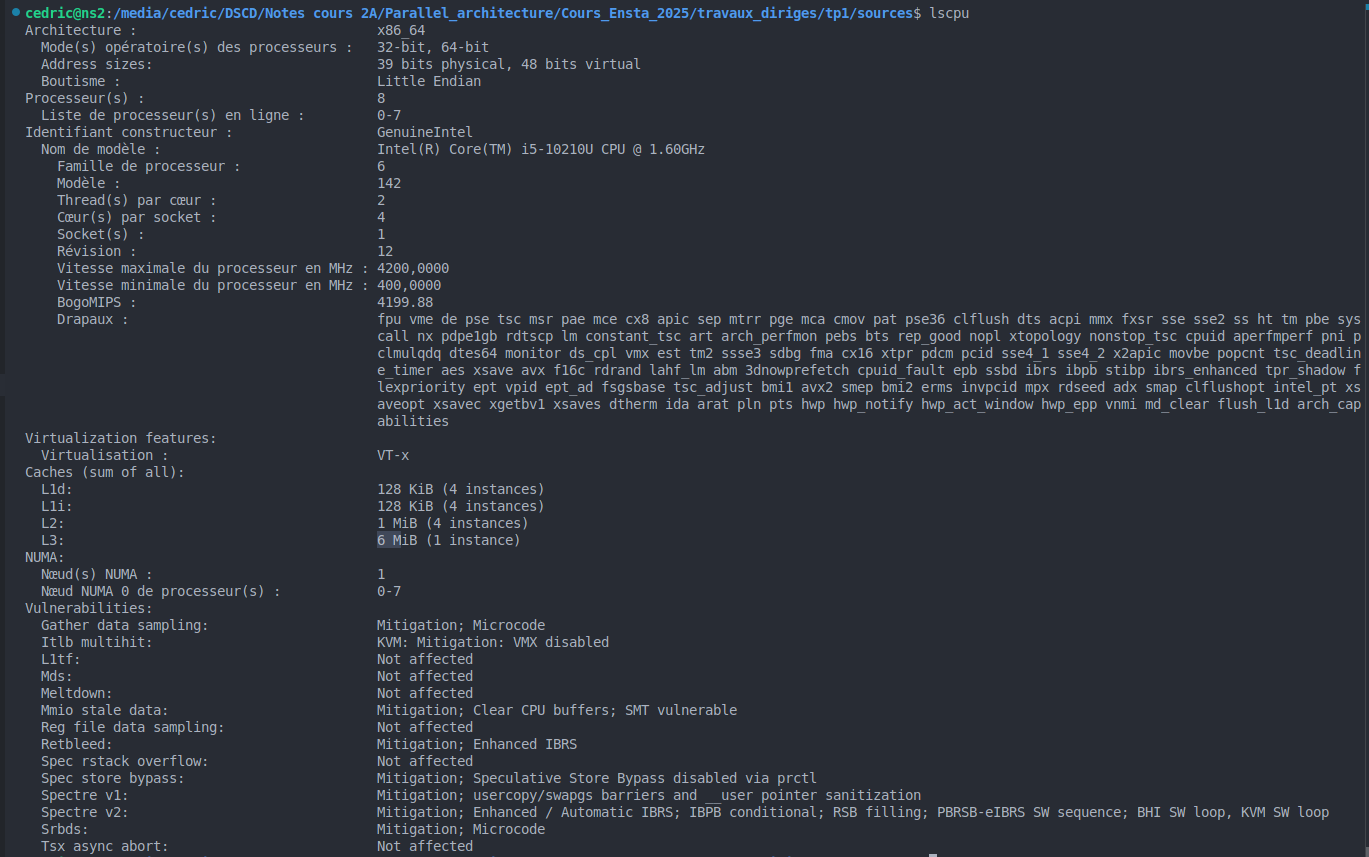
\includegraphics[scale=0.5]{images/lscpu.png}
    \caption{Résultat de la commande lscpu}
    \label{tab:lscpu}
\end{center}
\end{figure}


\begin{figure}[!h]
    \begin{center}
        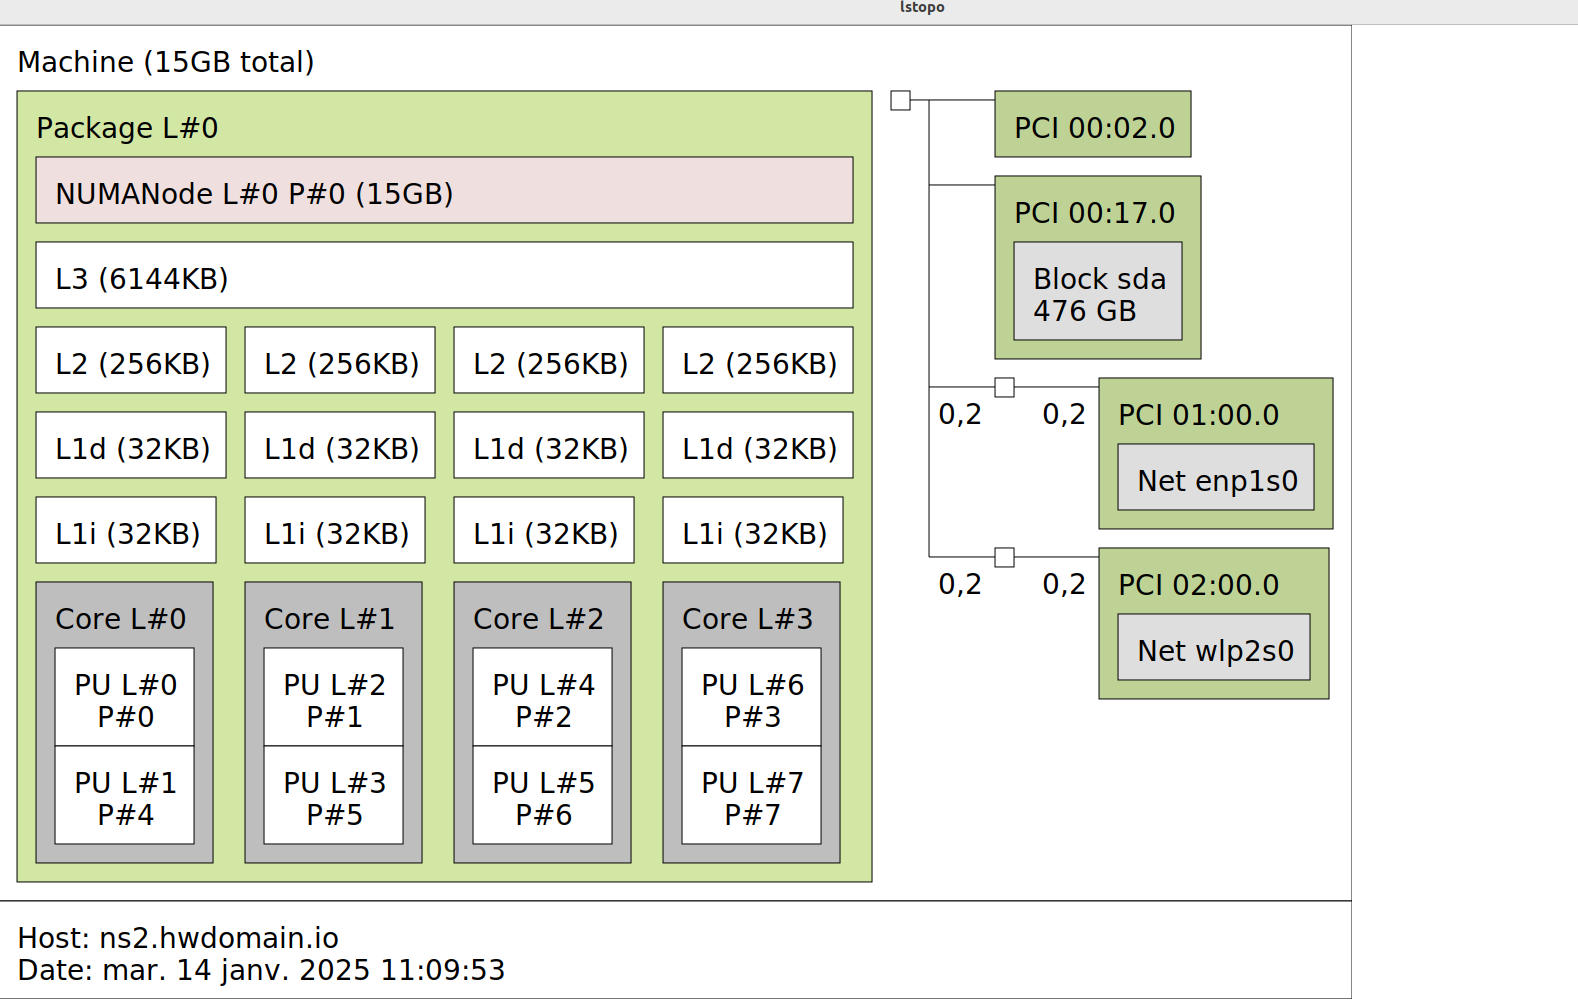
\includegraphics[scale=0.3]{images/lstopo.png}
        \caption{Résultat de la commande lstopo : Nous pouvons visualiser les tailles des caches}
        \label{tab:ls_topo}
    \end{center}
\end{figure}
\clearpage
\subsection{Comparer le temps pris par rapport au produit matrice–matrice "scalaire"}
    La version par bloc est significativement plus rapide grâce à une meilleure utilisation des caches. Pour une taille de blocs de \textbf{512}, et un thread, nous avons une durée de moyenne (pour les dimensions 1023, 1024 et 1025) de \textbf{0,564 secondes}  contre \textbf{1,537 secondes} pour le produit matrice-matrice scalaire.
\subsection{Parallélisation du produit matrice–matrice par bloc}
Code :  \\

	\begin{lstlisting}[language=C]
        Matrix operator*(const Matrix& A, const Matrix& B) {
            Matrix C(A.nbRows, B.nbCols, 0.0);
            const int szBlock = findOptimalBlockSize(A, B);
        
            #pragma omp parallel for
            for (int I = 0; I < A.nbRows; I += szBlock) {
                for (int J = 0; J < B.nbCols; J += szBlock) {
                    for (int K = 0; K < A.nbCols; K += szBlock) {
                        prodSubBlocks(I, J, K, szBlock, A, B, C);
                    }
                }
            }
            return C;
        }
\end{lstlisting}
\paragraph{Vérifions si la taille de bloc 512 reste optimale en variant le nombre de threads}
Les figures \ref{fig:execution_time_1}, \ref{fig:execution_time_4}, \ref{fig:execution_time_8} et \ref{fig:execution_time_16} nous montrent que à quelques exceptions près, la taille de bloc 512 nous fournit les meilleurs temps d'exécution.
\begin{table}[ht]
    \centering
    \caption{Temps d'exécution (secondes) pour N=1023--1025 et 2046--2050 (OMP\_NUM\_THREADS=1)}
    \label{tab:threads1}
    \begin{tabular}{|c|c|c|c|c|c|c|c|c|}\hline
    Taille & 16 & 32 & 64 & 128 & 256 & 512 & 1024 & 2048 \\\hline
    1023 & 0.793446 & 0.665258 & 0.635098 & 0.637810 & 0.573094 & \textbf{0.561053} & 0.725468 & 0.732480 \\\hline
    1024 & 0.886341 & 0.681334 & 0.628902 & 0.635453 & 0.567116 & \textbf{0.552188} & 0.706114 & 0.715358 \\\hline
    1025 & 0.801337 & 0.685229 & 0.630492 & 0.639878 & \textbf{0.574363} & 0.579971 & 0.733085 & 0.739268 \\\hline
    2046 & 6.439210 & 5.387410 & 4.786580 & 4.901310 & 4.598490 & \textbf{4.359200} & 6.310960 & 6.181470 \\\hline
    2048 & 8.126130 & 5.874090 & 5.053240 & 4.902760 & \textbf{4.416660} & 4.432710 & 6.007550 & 6.248670 \\\hline
    2050 & 6.606900 & 5.658080 & 5.137750 & 5.149390 & 4.777270 & \textbf{4.640320} & 6.353000 & 6.168310 \\\hline
    \end{tabular}
\end{table}


\begin{table}[ht]
    \centering
    \caption{Temps d'exécution (secondes) pour N=1023--1025 et 2046--2050 (OMP\_NUM\_THREADS=4)}
    \label{tab:threads4}
    \begin{tabular}{|c|c|c|c|c|c|c|c|c|}\hline
    Taille & 16 & 32 & 64 & 128 & 256 & 512 & 1024 & 2048 \\\hline
    1023 & 0.893265 & 0.710967 & 0.673102 & 0.687309 & 0.610476 & \textbf{0.597203} & 0.718978 & 0.721888 \\\hline
    1024 & 0.878508 & 0.702151 & 0.630565 & 0.642346 & 0.554412 & \textbf{0.572237} & 0.722451 & 0.721958 \\\hline
    1025 & 0.787681 & 0.683897 & 0.629180 & 0.620790 & 0.593019 & \textbf{0.569430} & 0.733281 & 0.726196 \\\hline
    2046 & 6.484090 & 5.388030 & 4.771340 & 4.863140 & 4.521920 & \textbf{4.354810} & 6.361110 & 6.156460 \\\hline
    2048 & 8.104590 & 5.852990 & 5.008800 & 4.935920 & \textbf{4.397090} & 4.335210 & 6.009580 & 6.201340 \\\hline
    2050 & 6.468300 & 5.497170 & 4.862740 & 4.899280 & 4.626760 & \textbf{4.536810} & 7.814800 & 6.157220 \\\hline
    \end{tabular}
\end{table}

\begin{table}[ht]
    \centering
    \caption{Temps d'exécution (secondes) pour N=1023--1025 et 2046--2050 (OMP\_NUM\_THREADS=8)}
    \label{tab:threads8}
    \begin{tabular}{|c|c|c|c|c|c|c|c|c|}\hline
    Taille & 16 & 32 & 64 & 128 & 256 & 512 & 1024 & 2048 \\\hline
    1023 & 0.821436 & 0.677631 & 0.628888 & 0.630129 & 0.576028 & \textbf{0.556613} & 0.728713 & 0.734240 \\\hline
    1024 & 0.883528 & 0.693663 & 0.627859 & 0.621725 & 0.562800 & \textbf{0.598684} & 0.725217 & 0.711722 \\\hline
    1025 & 0.804246 & 0.673618 & 0.621317 & 0.648724 & 0.598520 & \textbf{0.583687} & 0.739598 & 0.741214 \\\hline
    2046 & 6.487840 & 5.348190 & 4.750010 & 4.820080 & 4.515920 & \textbf{4.173970} & 6.126790 & 6.040050 \\\hline
    2048 & 9.409870 & 6.329540 & 7.120780 & 5.506070 & \textbf{5.147080} & 5.780910 & 9.244030 & 6.967800 \\\hline
    2050 & 6.795820 & 5.687700 & 5.042640 & 5.096350 & 4.772660 & \textbf{4.619370} & 6.553810 & 6.273280 \\\hline
    \end{tabular}
\end{table}
\begin{table}[ht]
    \centering
    \caption{Temps d'exécution (secondes) pour N=1023--1025 et 2046--2050 (OMP\_NUM\_THREADS=16)}
    \label{tab:threads16}
    \begin{tabular}{|c|c|c|c|c|c|c|c|c|}\hline
    Taille & 16 & 32 & 64 & 128 & 256 & 512 & 1024 & 2048 \\\hline
    1023 & 0.838795 & 0.696357 & 0.666950 & 0.674836 & 0.629240 & \textbf{0.610860} & 0.720595 & 0.720974 \\\hline
    1024 & 0.918404 & 0.713719 & 0.674944 & 0.652920 & 0.604920 & \textbf{0.586087} & 0.719093 & 0.717308 \\\hline
    1025 & 0.824739 & 0.688619 & 0.671568 & 0.685657 & 0.612800 & \textbf{0.594540} & 0.743956 & 0.740024 \\\hline
    2046 & 6.560780 & 5.401080 & 4.887390 & 4.881760 & 4.557290 & \textbf{4.376350} & 6.259490 & 6.093770 \\\hline
    2048 & 8.136170 & 5.905110 & 5.063990 & 5.015860 & 4.471350 & \textbf{4.386020} & 6.060130 & 6.269390 \\\hline
    2050 & 6.379520 & 6.049400 & 4.800330 & 4.951530 & 4.595810 & \textbf{4.423910} & 6.323920 & 6.200000 \\\hline
    \end{tabular}
\end{table}
    

    \begin{figure}[ht]
        \centering
        \begin{tikzpicture}
            \begin{axis}[
                xlabel={Taille des blocs},
                ylabel={Durée d'exécution (s)},
                grid=major,
                legend pos=north east,
                width=12cm,
                height=8cm
            ]
                % Courbe pour la taille 1023
                \addplot+[mark=o] table [x=Block, y=1023, col sep=comma] {data_threads1.csv};
                \addlegendentry{1023}
    
                % Courbe pour la taille 1024
                \addplot+[mark=square] table [x=Block, y=1024, col sep=comma] {data_threads1.csv};
                \addlegendentry{1024}
    
                % Courbe pour la taille 1025
                \addplot+[mark=triangle] table [x=Block, y=1025, col sep=comma] {data_threads1.csv};
                \addlegendentry{1025}
    
                % Courbe pour la taille 2046
                \addplot+[mark=diamond] table [x=Block, y=2046, col sep=comma] {data_threads1.csv};
                \addlegendentry{2046}
    
                % Courbe pour la taille 2048
                \addplot+[mark=pentagon] table [x=Block, y=2048, col sep=comma] {data_threads1.csv};
                \addlegendentry{2048}
    
                % Courbe pour la taille 2050
                \addplot+[mark=star] table [x=Block, y=2050, col sep=comma] {data_threads1.csv};
                \addlegendentry{2050}
            \end{axis}
        \end{tikzpicture}
        \caption{Durées d'exécution en fonction de la taille des blocs pour chaque taille de problème. (OMP\_NUM\_THREADS=1)}
        \label{fig:execution_time_1}
    \end{figure}
    \begin{figure}[ht]
        \centering
        \begin{tikzpicture}
            \begin{axis}[
                xlabel={Taille des blocs},
                ylabel={Durée d'exécution (s)},
                grid=major,
                legend pos=north east,
                width=12cm,
                height=8cm
            ]
                % Courbe pour la taille 1023
                \addplot+[mark=o] table [x=Block, y=1023, col sep=comma] {data_threads4.csv};
                \addlegendentry{1023}
    
                % Courbe pour la taille 1024
                \addplot+[mark=square] table [x=Block, y=1024, col sep=comma] {data_threads4.csv};
                \addlegendentry{1024}
    
                % Courbe pour la taille 1025
                \addplot+[mark=triangle] table [x=Block, y=1025, col sep=comma] {data_threads4.csv};
                \addlegendentry{1025}
    
                % Courbe pour la taille 2046
                \addplot+[mark=diamond] table [x=Block, y=2046, col sep=comma] {data_threads4.csv};
                \addlegendentry{2046}
    
                % Courbe pour la taille 2048
                \addplot+[mark=pentagon] table [x=Block, y=2048, col sep=comma] {data_threads4.csv};
                \addlegendentry{2048}
    
                % Courbe pour la taille 2050
                \addplot+[mark=star] table [x=Block, y=2050, col sep=comma] {data_threads4.csv};
                \addlegendentry{2050}
            \end{axis}
        \end{tikzpicture}
        \caption{Durées d'exécution en fonction de la taille des blocs pour chaque taille de problème. (OMP\_NUM\_THREADS=4)}
        \label{fig:execution_time_4}
    \end{figure}
    \begin{figure}[ht]
        \centering
        \begin{tikzpicture}
            \begin{axis}[
                xlabel={Taille des blocs},
                ylabel={Durée d'exécution (s)},
                grid=major,
                legend pos=north east,
                width=12cm,
                height=8cm
            ]
                % Courbe pour la taille 1023
                \addplot+[mark=o] table [x=Block, y=1023, col sep=comma] {data_threads8.csv};
                \addlegendentry{1023}
    
                % Courbe pour la taille 1024
                \addplot+[mark=square] table [x=Block, y=1024, col sep=comma] {data_threads8.csv};
                \addlegendentry{1024}
    
                % Courbe pour la taille 1025
                \addplot+[mark=triangle] table [x=Block, y=1025, col sep=comma] {data_threads8.csv};
                \addlegendentry{1025}
    
                % Courbe pour la taille 2046
                \addplot+[mark=diamond] table [x=Block, y=2046, col sep=comma] {data_threads8.csv};
                \addlegendentry{2046}
    
                % Courbe pour la taille 2048
                \addplot+[mark=pentagon] table [x=Block, y=2048, col sep=comma] {data_threads8.csv};
                \addlegendentry{2048}
    
                % Courbe pour la taille 2050
                \addplot+[mark=star] table [x=Block, y=2050, col sep=comma] {data_threads8.csv};
                \addlegendentry{2050}
            \end{axis}
        \end{tikzpicture}
        \caption{Durées d'exécution en fonction de la taille des blocs pour chaque taille de problème. (OMP\_NUM\_THREADS=8)}
        \label{fig:execution_time_8}
    \end{figure}

    \begin{figure}[ht]
        \centering
        \begin{tikzpicture}
            \begin{axis}[
                xlabel={Taille des blocs},
                ylabel={Durée d'exécution (s)},
                grid=major,
                legend pos=north east,
                width=12cm,
                height=8cm
            ]
                % Courbe pour la taille 1023
                \addplot+[mark=o] table [x=Block, y=1023, col sep=comma] {data_threads16.csv};
                \addlegendentry{1023}
    
                % Courbe pour la taille 1024
                \addplot+[mark=square] table [x=Block, y=1024, col sep=comma] {data_threads16.csv};
                \addlegendentry{1024}
    
                % Courbe pour la taille 1025
                \addplot+[mark=triangle] table [x=Block, y=1025, col sep=comma] {data_threads16.csv};
                \addlegendentry{1025}
    
                % Courbe pour la taille 2046
                \addplot+[mark=diamond] table [x=Block, y=2046, col sep=comma] {data_threads16.csv};
                \addlegendentry{2046}
    
                % Courbe pour la taille 2048
                \addplot+[mark=pentagon] table [x=Block, y=2048, col sep=comma] {data_threads16.csv};
                \addlegendentry{2048}
    
                % Courbe pour la taille 2050
                \addplot+[mark=star] table [x=Block, y=2050, col sep=comma] {data_threads16.csv};
                \addlegendentry{2050}
            \end{axis}
        \end{tikzpicture}
        \caption{Durées d'exécution en fonction de la taille des blocs pour chaque taille de problème. (OMP\_NUM\_THREADS=16)}
        \label{fig:execution_time_16}
    \end{figure}
\clearpage
\paragraph{Mesure de l'accélération}
Dans cette section, nous nous concentrons uniquement sur les tailles de blocs \textbf{256} et \textbf{512} car ce sont les seules qui conduisent à des temps d'exécution minimaux. Pour chacune de ces tailles, nous avons calculé la moyenne des temps CPU mesurés sur les six dimensions testées (N = 1023, 1024, 1025, 2046, 2048, 2050) pour chaque configuration de threads (OMP\_NUM\_THREADS = 1, 4, 8, 16). La moyenne obtenue pour le cas 1 thread sert de référence pour calculer l'accélération (speedup) selon la formule suivante :

\[
\text{Speedup} = \frac{T_{\text{moyenne}}(1 \text{ thread})}{T_{\text{moyenne}}(n \text{ threads})}.
\]

\subparagraph*{Taille de bloc 256}

Les moyennes des temps CPU obtenues sont les suivantes :
\begin{itemize}
    \item OMP\_NUM\_THREADS = 1 : \(T_{1}(256) \approx 2.58\,\text{s}\)
    \item OMP\_NUM\_THREADS = 4 : \(T_{4}(256) \approx 2.55\,\text{s}\)
    \item OMP\_NUM\_THREADS = 8 : \(T_{8}(256) \approx 2.70\,\text{s}\)
    \item OMP\_NUM\_THREADS = 16 : \(T_{16}(256) \approx 2.58\,\text{s}\)
\end{itemize}

Les accélérations correspondantes sont alors :
\begin{itemize}
    \item 1 thread : Speedup = \(1.00\) (référence)
    \item 4 threads : Speedup \(\approx \frac{2.58}{2.55} \approx 1.01\)
    \item 8 threads : Speedup \(\approx \frac{2.58}{2.70} \approx 0.96\)
    \item 16 threads : Speedup \(\approx \frac{2.58}{2.58} \approx 1.00\)
\end{itemize}

\subparagraph*{Taille de bloc 512}

Les moyennes des temps CPU obtenues pour la taille de bloc 512 sont :
\begin{itemize}
    \item OMP\_NUM\_THREADS = 1 : \(T_{1}(512) \approx 2.52\,\text{s}\)
    \item OMP\_NUM\_THREADS = 4 : \(T_{4}(512) \approx 2.49\,\text{s}\)
    \item OMP\_NUM\_THREADS = 8 : \(T_{8}(512) \approx 2.72\,\text{s}\)
    \item OMP\_NUM\_THREADS = 16 : \(T_{16}(512) \approx 2.50\,\text{s}\)
\end{itemize}

Les accélérations correspondantes sont :
\begin{itemize}
    \item 1 thread : Speedup = \(1.00\) (référence)
    \item 4 threads : Speedup \(\approx \frac{2.52}{2.49} \approx 1.01\)
    \item 8 threads : Speedup \(\approx \frac{2.52}{2.72} \approx 0.93\)
    \item 16 threads : Speedup \(\approx \frac{2.52}{2.50} \approx 1.01\)
\end{itemize}
\subparagraph*{Tableau récapitulatif des accélérations pour les tailles de blocs 256 et 512}
\begin{table}[ht]
    \centering
    \caption{Accélérations moyennes (baseline : OMP\_NUM\_THREADS = 1) pour les tailles de blocs 256 et 512}
    \label{tab:speedup256512}
    \begin{tabular}{|c|c|c|c|c|}
        \hline
        Taille de bloc & 1 thread & 4 threads & 8 threads & 16 threads \\ \hline
        256          & 1.00     & 1.01      & 0.96      & 1.00       \\ \hline
        512          & 1.00     & 1.01      & 0.93      & 1.01       \\ \hline
    \end{tabular}
\end{table}
Pour une taille de bloc fixée, nous représentons l'évolution de l'accélération (speedup) en fonction du nombre de threads.
\subparagraph*{Évolution des accélérations pour la taille de bloc 256}

\begin{figure}[ht]
    \centering
    \begin{tikzpicture}
        \begin{axis}[
            width=0.7\textwidth,
            height=0.5\textwidth,
            xlabel={Nombre de threads},
            ylabel={Accélération (speedup)},
            xmin=0, xmax=20,
            ymin=0.8, ymax=1.1,
            xtick={1,4,8,16},
            ytick={0.8,0.9,1.0,1.1},
            grid=both,
            grid style={line width=.1pt, draw=gray!10},
            major grid style={line width=.2pt,draw=gray!50},
            legend pos=south east,
            legend cell align={left}
        ]
        \addplot[
            color=blue,
            mark=*,
            smooth,
        ]
        table[col sep=comma]{data256.csv};
        \addlegendentry{Bloc 256}
        \end{axis}
    \end{tikzpicture}
    \caption{Évolution du speedup en fonction du nombre de threads pour une taille de bloc de 256.}
    \label{fig:speedup256}
\end{figure}

\subparagraph*{Évolution des accélérations pour la taille de bloc 512}

\begin{figure}[ht]
    \centering
    \begin{tikzpicture}
        \begin{axis}[
            width=0.7\textwidth,
            height=0.5\textwidth,
            xlabel={Nombre de threads},
            ylabel={Accélération (speedup)},
            xmin=0, xmax=20,
            ymin=0.8, ymax=1.1,
            xtick={1,4,8,16},
            ytick={0.8,0.9,1.0,1.1},
            grid=both,
            grid style={line width=.1pt, draw=gray!10},
            major grid style={line width=.2pt,draw=gray!50},
            legend pos=south east,
            legend cell align={left}
        ]
        \addplot[
            color=red,
            mark=square*,
            smooth,
        ]
        table[col sep=comma]{data512.csv};
        \addlegendentry{Bloc 512}
        \end{axis}
    \end{tikzpicture}
    \caption{Évolution du speedup en fonction du nombre de threads pour une taille de bloc de 512.}
    \label{fig:speedup512}
\end{figure}

\textbf{Remarques :}
\begin{itemize}
    \item Pour la taille de bloc 256, une légère amélioration est observée avec 4 threads (speedup \(\approx 1.01\)) et 16 threads (speedup \(\approx 1.00\)), tandis que 8 threads présente une performance légèrement inférieure (speedup \(\approx 0.96\)).
    \item Pour la taille de bloc 512, on note également une amélioration avec 4 et 16 threads (speedup \(\approx 1.01\)), et une dégradation avec 8 threads (speedup \(\approx 0.93\)).
\end{itemize}
\textbf{Commentaire :}
\begin{itemize}
    \item Avec 4 threads : amélioration légère (speedup $\approx 1.01$)

    Chaque thread peut s'exécuter sur un c\oe ur distinct sans entrer en conflit avec un autre thread.

    \item Avec 8 threads : légère dégradation (speedup $\approx 0.96$ pour 256, $\approx 0.93$ pour 512)

    L'Hyper-Threading crée une compétition entre les threads d’un même c\oe ur, ce qui peut augmenter les latences d'accès au cache.
    L'augmentation du nombre de threads entraîne une saturation des unités d’exécution et des ressources mémoire.

\end{itemize}
\clearpage
\paragraph{Comparaison avec le produit matrice-matrice "scalaire"}
\begin{enumerate}
\item \textbf{ Observation} :
L'accélération parallèle est inférieure pour la version par blocs.
\item \textbf{Explications }:
    \begin{itemize}
        \item 
    \end{itemize}
\end{enumerate}
\textbf{Raison }:
Le surcoût de synchronisation est amorti par le volume de calcul dans chaque bloc.
 \subsection{Comparaison avec BLAS} 

 \begin{table}[h!]
    \begin{center}
    \begin{tabular}{|c|c|c|}
        \hline
        Dimension & Temps CPU (s) & MFlops \\ \hline
        1023      & 0.0473309       & 45238.9 \\ \hline
        1024      & 0.0609969       & 35206.4 \\ \hline
        1025      & 0.057084       & 37730 \\ \hline
        Moyenne & 0.055 & 39391,77 \\ \hline
    \end{tabular}
    \caption{Temps de calcul et performances en MFlops pour différentes dimensions de matrices obtenus avec Blas.}
    \label{tab:perf_matrix}
\end{center}
\end{table}
Les performances obtenues avec BLAS sont meilleures que celles obtenues avec notre produit matrice matrice par blocs parallélisé (16 threads). Le rapport moyen des performances $\approx \frac{0,247}{0.055} = 4.49$.

La meilleure version est celle de BLAS.
\section{Parallélisation MPI}
\subsection{Circulation d'un jeton dans un anneau.}


Code : \\

	\begin{lstlisting}[language=C]

        #include <stdio.h>
        #include <mpi.h>
        
        int main(int argc, char *argv[]) {
            int rank, nbp, token;
        
            /* Initialisation de l'environnement MPI */
            MPI_Init(&argc, &argv);
            MPI_Comm_rank(MPI_COMM_WORLD, &rank);
            MPI_Comm_size(MPI_COMM_WORLD, &nbp);
        
            /* On verifie qu'il y a au moins 2 processus */
            if(nbp < 2) {
                if(rank == 0)
                    fprintf(stderr, "Ce programme necessite au moins 2 processus.\n");
                MPI_Finalize();
                return 1;
            }
        
            /* Processus de rang 0 initialise le jeton et l'envoie au processus de rang 1 */
            if (rank == 0) {
                token = 1;  // initialisation du jeton
                printf("Processus %d envoie le jeton %d vers le processus 1\n", rank, token);
                MPI_Send(&token, 1, MPI_INT, 1, 0, MPI_COMM_WORLD);
                
                /* Processus 0 attend ensuite de recevoir le jeton venant du dernier processus */
                MPI_Recv(&token, 1, MPI_INT, nbp - 1, 0, MPI_COMM_WORLD, MPI_STATUS_IGNORE);
                printf("Processus %d a reçu le jeton %d depuis le processus %d\n", rank, token, nbp - 1);
            }
            else {
                /* Tous les autres processus reçoivent le jeton du processus precedent */
                MPI_Recv(&token, 1, MPI_INT, rank - 1, 0, MPI_COMM_WORLD, MPI_STATUS_IGNORE);
                token++;  // incrementation du jeton
                printf("Processus %d a reçu le jeton et l'incremente à %d\n", rank, token);
        
                /* Envoi du jeton au processus suivant.
                   Le processus nbp-1 envoie vers le processus 0 pour fermer l'anneau. */
                int dest = (rank + 1) % nbp;
                MPI_Send(&token, 1, MPI_INT, dest, 0, MPI_COMM_WORLD);
            }
        
            MPI_Finalize();
            return 0;
        }
        
\end{lstlisting}

\paragraph{Exécution}
\begin{enumerate}
    \item mpicc jeton.c -o jeton
    \item mpirun -np 4 ./jeton
\end{enumerate}
4 étant la valeur de nbp.\\
\textbf{Résultat}
\begin{itemize}
\item Processus 0 envoie le jeton 1 vers le processus 1
\item Processus 1 a reçu le jeton et l'incrémente à 2
\item Processus 2 a reçu le jeton et l'incrémente à 3
\item Processus 3 a reçu le jeton et l'incrémente à 4
\item Processus 0 a reçu le jeton 4 depuis le processus 3
\end{itemize}
\subsubsection{Calcul très approché de \pi}
\paragraph{Version séquentielle en c}.\\

	\begin{lstlisting}[language=C]
        /* pi_seq.c */
        #include <stdio.h>
        #include <stdlib.h>
        #include <time.h>
        #include <math.h>
        
        double approximate_pi(unsigned long nbSamples) {
            unsigned long nbDarts = 0;
            for (unsigned long i = 0; i < nbSamples; i++) {
                /* Generer un point dans [-1, 1] */
                double x = (double)rand() / RAND_MAX * 2.0 - 1.0;
                double y = (double)rand() / RAND_MAX * 2.0 - 1.0;
                if (x*x + y*y <= 1.0)
                    nbDarts++;
            }
            double ratio = (double)nbDarts / nbSamples;
            return 4.0 * ratio;
        }
        
        int main(void) {
            unsigned long nbSamples = 10000000UL; // par exemple 10 millions de points
            srand(time(NULL));
            clock_t tdeb = clock();
            double pi = approximate_pi(nbSamples);
            clock_t tfin = clock();
            double temps = (double)(tfin - tdeb) / CLOCKS_PER_SEC;
            printf("Approximation de pi (sequentiel) = %f\n", pi);
            printf("Temps d'execution = %f secondes\n", temps);
            return 0;
        }
        
        
\end{lstlisting}

\paragraph{Paralléliser en mémoire partagée le programme séquentiel en C à l'aide d’OpenMP}.\\


	\begin{lstlisting}[language=C]
        /* pi_openmp.c */
        #include <stdio.h>
        #include <stdlib.h>
        #include <time.h>
        #include <math.h>
        #include <omp.h>
        
        double approximate_pi(unsigned long nbSamples) {
            unsigned long nbDarts = 0;
        
            #pragma omp parallel
            {
                unsigned int seed = time(NULL) ^ omp_get_thread_num(); 
                unsigned long localCount = 0;
                #pragma omp for
                for (unsigned long i = 0; i < nbSamples; i++) {
                    double x = (double)rand_r(&seed) / RAND_MAX * 2.0 - 1.0;
                    double y = (double)rand_r(&seed) / RAND_MAX * 2.0 - 1.0;
                    if (x*x + y*y <= 1.0)
                        localCount++;
                }
                #pragma omp atomic
                nbDarts += localCount;
            }
            double ratio = (double)nbDarts / nbSamples;
            return 4.0 * ratio;
        }
        
        int main(void) {
            unsigned long nbSamples = 10000000UL;
            double tdeb = omp_get_wtime();
            double pi = approximate_pi(nbSamples);
            double tfin = omp_get_wtime();
            printf("Approximation de pi (OpenMP) = %f\n", pi);
            printf("Temps d'execution = %f secondes\n", tfin - tdeb);
            return 0;
        }
        
\end{lstlisting}

\paragraph{Mesure de l'accélération (fig \ref{tab:pi_approximation})}
\begin{table}[h!]
    \centering
    \begin{tabular}{|c|c|c|c|}
        \hline
    \toprule
    \textbf{Nombre de threads} & \textbf{Approximation de $\pi$ (OpenMP)} & \textbf{Temps d'exécution (secondes)} & \textbf{Accélération}\\
    \midrule
    1 thread                  & 3.141976                                  & 0.118586        & 1                       \\\hline
    4 threads                 & 3.142339                                  & 0.055988         &    2,118061013                  \\\hline
    8 threads                 & 3.140559                                  & 0.054829           & 2,162833537                   \\\hline
    16 threads                 & 3.141930                                  &  0.04843           & 2,448606236                   \\\hline
    \bottomrule
    \end{tabular}
    \caption{Résultats de l'approximation de $\pi$ avec OpenMP pour différents nombres de threads.}
    \label{tab:pi_approximation}
    \end{table}

    \paragraph{Version en mémoire distribuée avec MPI en C}.\\
    \begin{lstlisting}[language=C][language=C, caption=Code source de \texttt{pi\_mpi.c}]
        /* pi_mpi.c */
        #include <stdio.h>
        #include <stdlib.h>
        #include <time.h>
        #include <math.h>
        #include <mpi.h>
        
        int main(int argc, char *argv[]) {
            int rank, nbp;
            MPI_Init(&argc, &argv);
            MPI_Comm_rank(MPI_COMM_WORLD, &rank);
            MPI_Comm_size(MPI_COMM_WORLD, &nbp);
        
            unsigned long nbSamplesTotal = 10000000UL;
            /* Chaque processus traite une portion des echantillons */
            unsigned long nbSamples = nbSamplesTotal / nbp;
            unsigned long nbDarts_local = 0;
        
            /* Utiliser une graine differente pour chaque processus */
            unsigned int seed = time(NULL) ^ rank;
        
            double tdeb = MPI_Wtime();
            for (unsigned long i = 0; i < nbSamples; i++) {
                double x = (double)rand_r(&seed) / RAND_MAX * 2.0 - 1.0;
                double y = (double)rand_r(&seed) / RAND_MAX * 2.0 - 1.0;
                if (x*x + y*y <= 1.0)
                    nbDarts_local++;
            }
        
            unsigned long nbDarts_total = 0;
            MPI_Reduce(&nbDarts_local, &nbDarts_total, 1, MPI_UNSIGNED_LONG, MPI_SUM, 0, MPI_COMM_WORLD);
            double tfin = MPI_Wtime();
        
            if (rank == 0) {
                double ratio = (double)nbDarts_total / (nbSamples * nbp);
                double pi = 4.0 * ratio;
                printf("Approximation de pi (MPI) = %f\n", pi);
                printf("Temps d'execution (MPI) = %f secondes\n", tfin - tdeb);
            }
        
            MPI_Finalize();
            return 0;
        }        
        
\end{lstlisting}

\paragraph{Mesure de l'accélération (fig \ref{tab:pi_mpi})}


    \begin{table}[h!]
        \centering
        \begin{tabular}{|c|c|c|c|}
        \hline
        \textbf{Nombre de processus} & \textbf{Approximation de $\pi$ (MPI)} & \textbf{Temps d'exécution (secondes)} & \textbf{Accélération} \\
        \hline
        1                           & 3.141547                              & 0.168330                  & 1 \\\hline
        2                           & 3.141825                              & 0.084710                 &    1,98713257          \\\hline
        4                           & 3.142389                              & 0.072163                   &     2,332635838       \\\hline
        6                           & \textit{Erreur}                       & \textit{Non disponible}      & Non disponible         \\\hline
        8                           & \textit{Erreur}                       & \textit{Non disponible}      & Non disponible         \\\hline
        \end{tabular}
        \caption{Résultats de l'approximation de $\pi$ avec MPI pour différents nombres de processus.}
        \label{tab:pi_mpi}
        \end{table}
    
    \paragraph{Commentaire }
    Causes des erreurs : 
    \item Nombre de slots disponibles insuffisant
    \begin{itemize}
    \item Open MPI utilise le concept de slots pour allouer des processus. Un slot correspond à une unité d'allocation (généralement un cœur ou un thread).
    \item Notre processeur (Intel Core i5-10210U) a 4 cœurs physiques et 8 threads logiques (grâce à la technologie Hyper-Threading (fig \ref{tab:lscpu})).
    \item Par défaut, Open MPI limite le nombre de slots au nombre de cœurs physiques ou threads disponibles. Si on essaie de lancer plus de processus que de slots disponibles, l'erreur se produit.
    \end{itemize}
\paragraph{Version MPI en python avec mpi4py}.\\

	\begin{lstlisting}[language=C]
        #!/usr/bin/env python3
        # pi_mpi.py
        from mpi4py import MPI
        import time, numpy as np
        
        comm = MPI.COMM_WORLD
        rank = comm.Get_rank()
        size = comm.Get_size()
        
        nb_samples_total = 40_000_000
        nb_samples = nb_samples_total // size  # repartition uniforme des echantillons
        
        # Debut de la mesure de temps (commence avant le calcul)
        start = MPI.Wtime()
        
        # Chaque processus initialise sa graine pour générer des nombres aleatoires différents
        np.random.seed(int(time.time()) ^ rank)
        
        # Generation des points aleatoires dans [-1, 1] pour x et y
        x = np.random.uniform(-1, 1, nb_samples)
        y = np.random.uniform(-1, 1, nb_samples)
        
        # Compter le nombre de points tombant dans le cercle unite
        local_count = np.count_nonzero(x*x + y*y <= 1.0)
        
        # Réduire les resultats de tous les processus (somme)
        total_count = comm.reduce(local_count, op=MPI.SUM, root=0)
        
        # Fin de la mesure de temps
        end = MPI.Wtime()
        
        # Le processus maitre calcule l'approximation de pi et affiche le temps d'execution
        if rank == 0:
            approx_pi = 4.0 * total_count / nb_samples_total
            print(f"Approximation de pi (mpi4py) = {approx_pi}")
            print(f"Temps d'execution = {end - start} secondes")
        
        
\end{lstlisting}

\begin{table}[h!]
    \centering
    \begin{tabular}{|c|c|c|c|}
    \toprule
    \hline
    \textbf{Nombre de processus} & \textbf{Approximation de $\pi$ (MPI)} & \textbf{Temps d'exécution (secondes)} & \textbf{Accélération}\\
    \midrule    
    \hline
    1                           & 3.141979                              & 1.43688583   & 1                              \\\hline
    2                           & 3.1421147                              & 0.709724572     &    2,024568243                       \\\hline
    4                           & 3.1417664                              & 0.684759401      &     2,098380581                    \\\hline
    6                           & \textit{Erreur}                       & \textit{Non disponible}    & Non disponible            \\\hline
    8                           & \textit{Erreur}                       & \textit{Non disponible}    & Non disponible           \\\hline
    \bottomrule
    \end{tabular}
    \caption{Résultats de l'approximation de $\pi$ avec MPI pour différents nombres de processus.}
    \label{tab:pi_mpi_py}
    \end{table}

\subsection{Diffusion d'un entier dans un réseau hypercube.  }
Code :  \\


	\begin{lstlisting}[language=C]
        #include <stdio.h>
        #include <stdlib.h>
        #include <mpi.h>
        
        int main(int argc, char* argv[]) {
            int rank, nbp, d;
            MPI_Init(&argc, &argv);
            MPI_Comm_rank(MPI_COMM_WORLD, &rank);
            MPI_Comm_size(MPI_COMM_WORLD, &nbp);
        
            // Determination de la dimension d :
            // Si un argument est fourni, on l'utilise ; sinon, on deduit d a partir du nb de processus.
            if (argc > 1) {
                d = atoi(argv[1]);
            } else {
                // Deduire d si nbp est une puissance de 2.
                d = 0;
                int tmp = nbp;
                while (tmp > 1) {
                    if (tmp % 2 != 0) {
                        if (rank == 0)
                            fprintf(stderr, "Erreur : Le nombre de processus doit etre une puissance de 2.\n");
                        MPI_Finalize();
                        exit(EXIT_FAILURE);
                    }
                    tmp /= 2;
                    d++;
                }
            }
        
            // Verification : le nombre de processus doit etre 2^d.
            if (nbp != (1 << d)) {
                if (rank == 0)
                    fprintf(stderr, "Erreur : Pour un hypercube de dimension %d, il faut 2^d processus (ici %d processus).\n", d, nbp);
                MPI_Finalize();
                exit(EXIT_FAILURE);
            }
        
            int token;  // le jeton a diffuser
            double tdeb, tfin;
            
            // Mesurer le temps de diffusion
            tdeb = MPI_Wtime();
        
            // 1. Cas de l'hypercube de dimension 1 (2 processus) :
            //    - Si d vaut 1, alors seul 2 processus sont utilises.
            //    - Le processus 0 initialise et envoie au processus 1.
            // Ce meme algorithme fonctionne pour d = 2, d = 3 et d = d general.
            if (rank == 0) {
                token = 12345;  // valeur choisie par le programmeur
            }
            
            // Diffusion dans un hypercube en d etapes.
            // Pour chaque etape i, chaque processus echange avec son partenaire defini par rank xor (1 << i).
            for (int i = 0; i < d; i++) {
                int partner = rank ^ (1 << i);
                if (rank < partner) {
                    // Le processus avec un rang plus faible envoie d'abord
                    MPI_Send(&token, 1, MPI_INT, partner, 0, MPI_COMM_WORLD);
                } else {
                    // Celui avec le rang plus eleve recoit
                    MPI_Recv(&token, 1, MPI_INT, partner, 0, MPI_COMM_WORLD, MPI_STATUS_IGNORE);
                }
            }
            
            tfin = MPI_Wtime();
        
            // Affichage : chaque processus affiche la valeur recue et le temps de diffusion.
            printf("Processus %d : token = %d, temps de diffusion = %f secondes\n", rank, token, tfin - tdeb);
        
            MPI_Finalize();
            return 0;
        }
        
\end{lstlisting}
\textbf{mpirun -np 4 ./compute\_hypercube 2}
\begin{itemize}
\item Processus 0 : token = 12345, temps de diffusion = 0.000027 secondes
\item Processus 1 : token = 12345, temps de diffusion = 0.000085 secondes
\item Processus 2 : token = 12345, temps de diffusion = 0.000027 secondes
\item Processus 3 : token = 12345, temps de diffusion = 0.000116 secondes
\end{itemize}
\begin{know}
Faire varier les tailles des caches et voir le point à partir duquel ça décroit


à un moment donnée il faut qu'on fasse entre 3 fois la taille d'un bloc soit bloc\_size * block\_size * 8 * 3  et comparer ceci à la taille des caches L1, L2, L3


vérifier si la taille des blocs en monothreadé est optimale en multithreadé

BLAS est disponible dans plusieurs versions. OpenBlas et KL sont optimisées. celle de notre machine ne l'est pas forcément.

apt install libmkl-dev (l'alternative c'est openblas)

Quand on fait mpirun -nb 4 mon\_prog, il lance 4 instance de mon\_prog et puis il les mets sur 4 corps différents. Chaque instance du programme doit savoir qu'elle place elle a dans le programme pour savoir ce qu'elle doit faire. On peut voir la programation mpi comme un jeu de role et le role est déterminé par le rank. La commande mpirun lance chaque instance du programme dans un contexte d'exécution spécifique en attribuant à chacun un rank. Get\_rank nous permet d'avoir le rank. Quand on fait un programme MPI, on doit se dire qu'on a un seul programme et la seule façon de faire des roles différents est de faire des comparaisons sur le rank.

question 1 tD2:  pb déséquilibrage des charges car le calcul de chaque point n'a pas la meme complexité. 

Premier point : analyse macroscopique du code pour cibler les étapes les plus couteuses.

Quand on découpe la fractale en 2 (sur l'axe x), on n'a pas de déséquilibrage des charges. 

le temps de calcul de la fractale sur chaque processeur  nous permettra de savoir si on a un déséquilibrage ou non

le temps d'une communication = ttemps d'initialisation (incompressible) + temps de transfert, ainsi l'approche pixel par pixel n'est pas viable.

il faut donc faire le moins de communications possibles 

il faut trouver un équilibre entre une Granularité trop faible et trop grosse

le maitre esclave semble etre viable(on le fait surtout quand on ne sait pas à priori comment repartir les chargese) 

faire des dessins pour voir comment les données sont parcourues et cela permettra de voir comment les distribuer.

produit matrice vecteur : 

le mpi broadcast nous permet de partage une informatioin à plusieurs processus.

le mpi getter nous permet de rassembler plusieurs informations 

mpi allgather fait un getter suivi d'un broadcast

mpi scatter permet de découper une variable et envoyer sur chaque processus 

mpi reduce (necessite un processeur cible)

mpi allreduce (n'en necessite pas et est un reduce ssuivi d'un broadcast)
\end{know}
\end{document}



